\documentclass[12pt,titlepage]{article}

\setlength{\oddsidemargin}{0in}
\setlength{\evensidemargin}{0in}
\setlength{\textwidth}{6.5in}
%
\setlength{\textheight}{9in}
\setlength{\topmargin}{0in}
\setlength{\headsep}{0in}
\setlength{\topskip}{0in}
\setlength{\headheight}{0in}

\usepackage{graphicx}
\usepackage{times}
\usepackage[plainpages=false, colorlinks=true, anchorcolor=blue, linkcolor=blue, citecolor=blue, bookmarks=false, urlcolor=blue]
{hyperref}
\usepackage[square,comma,authoryear]{natbib}


\title{DOE Office of Science INCITE Project:\\
{\it Extreme-scale Simulation of Supernovae and Magnetars from Realistic Progenitors}\\
2018 Q1 Report}

\author{Principal Investigator:\\Sean M. Couch\\
  Michigan State University \vspace{0.1in}\\
  Co-Investigators: \\
  Andrew Christlieb (Michigan State University) \\
  Evan O'Connor (Stockholm University)\\
  Kuo-Chuan Pan (Michigan State University) \\
  Luke Roberts (Michigan State University) \\
  MacKenzie Warren (Michigan State University) \\
}

\date{April 1, 2018}


\begin{document}


\maketitle


%%%%%%%%%%%%%%%%%%%%%%%%%%%%%%%%%
\section{Project Usage}

%%%%%%%%%%%%%%%%%%%


\begin{figure}
  \begin{tabular}{cc}
    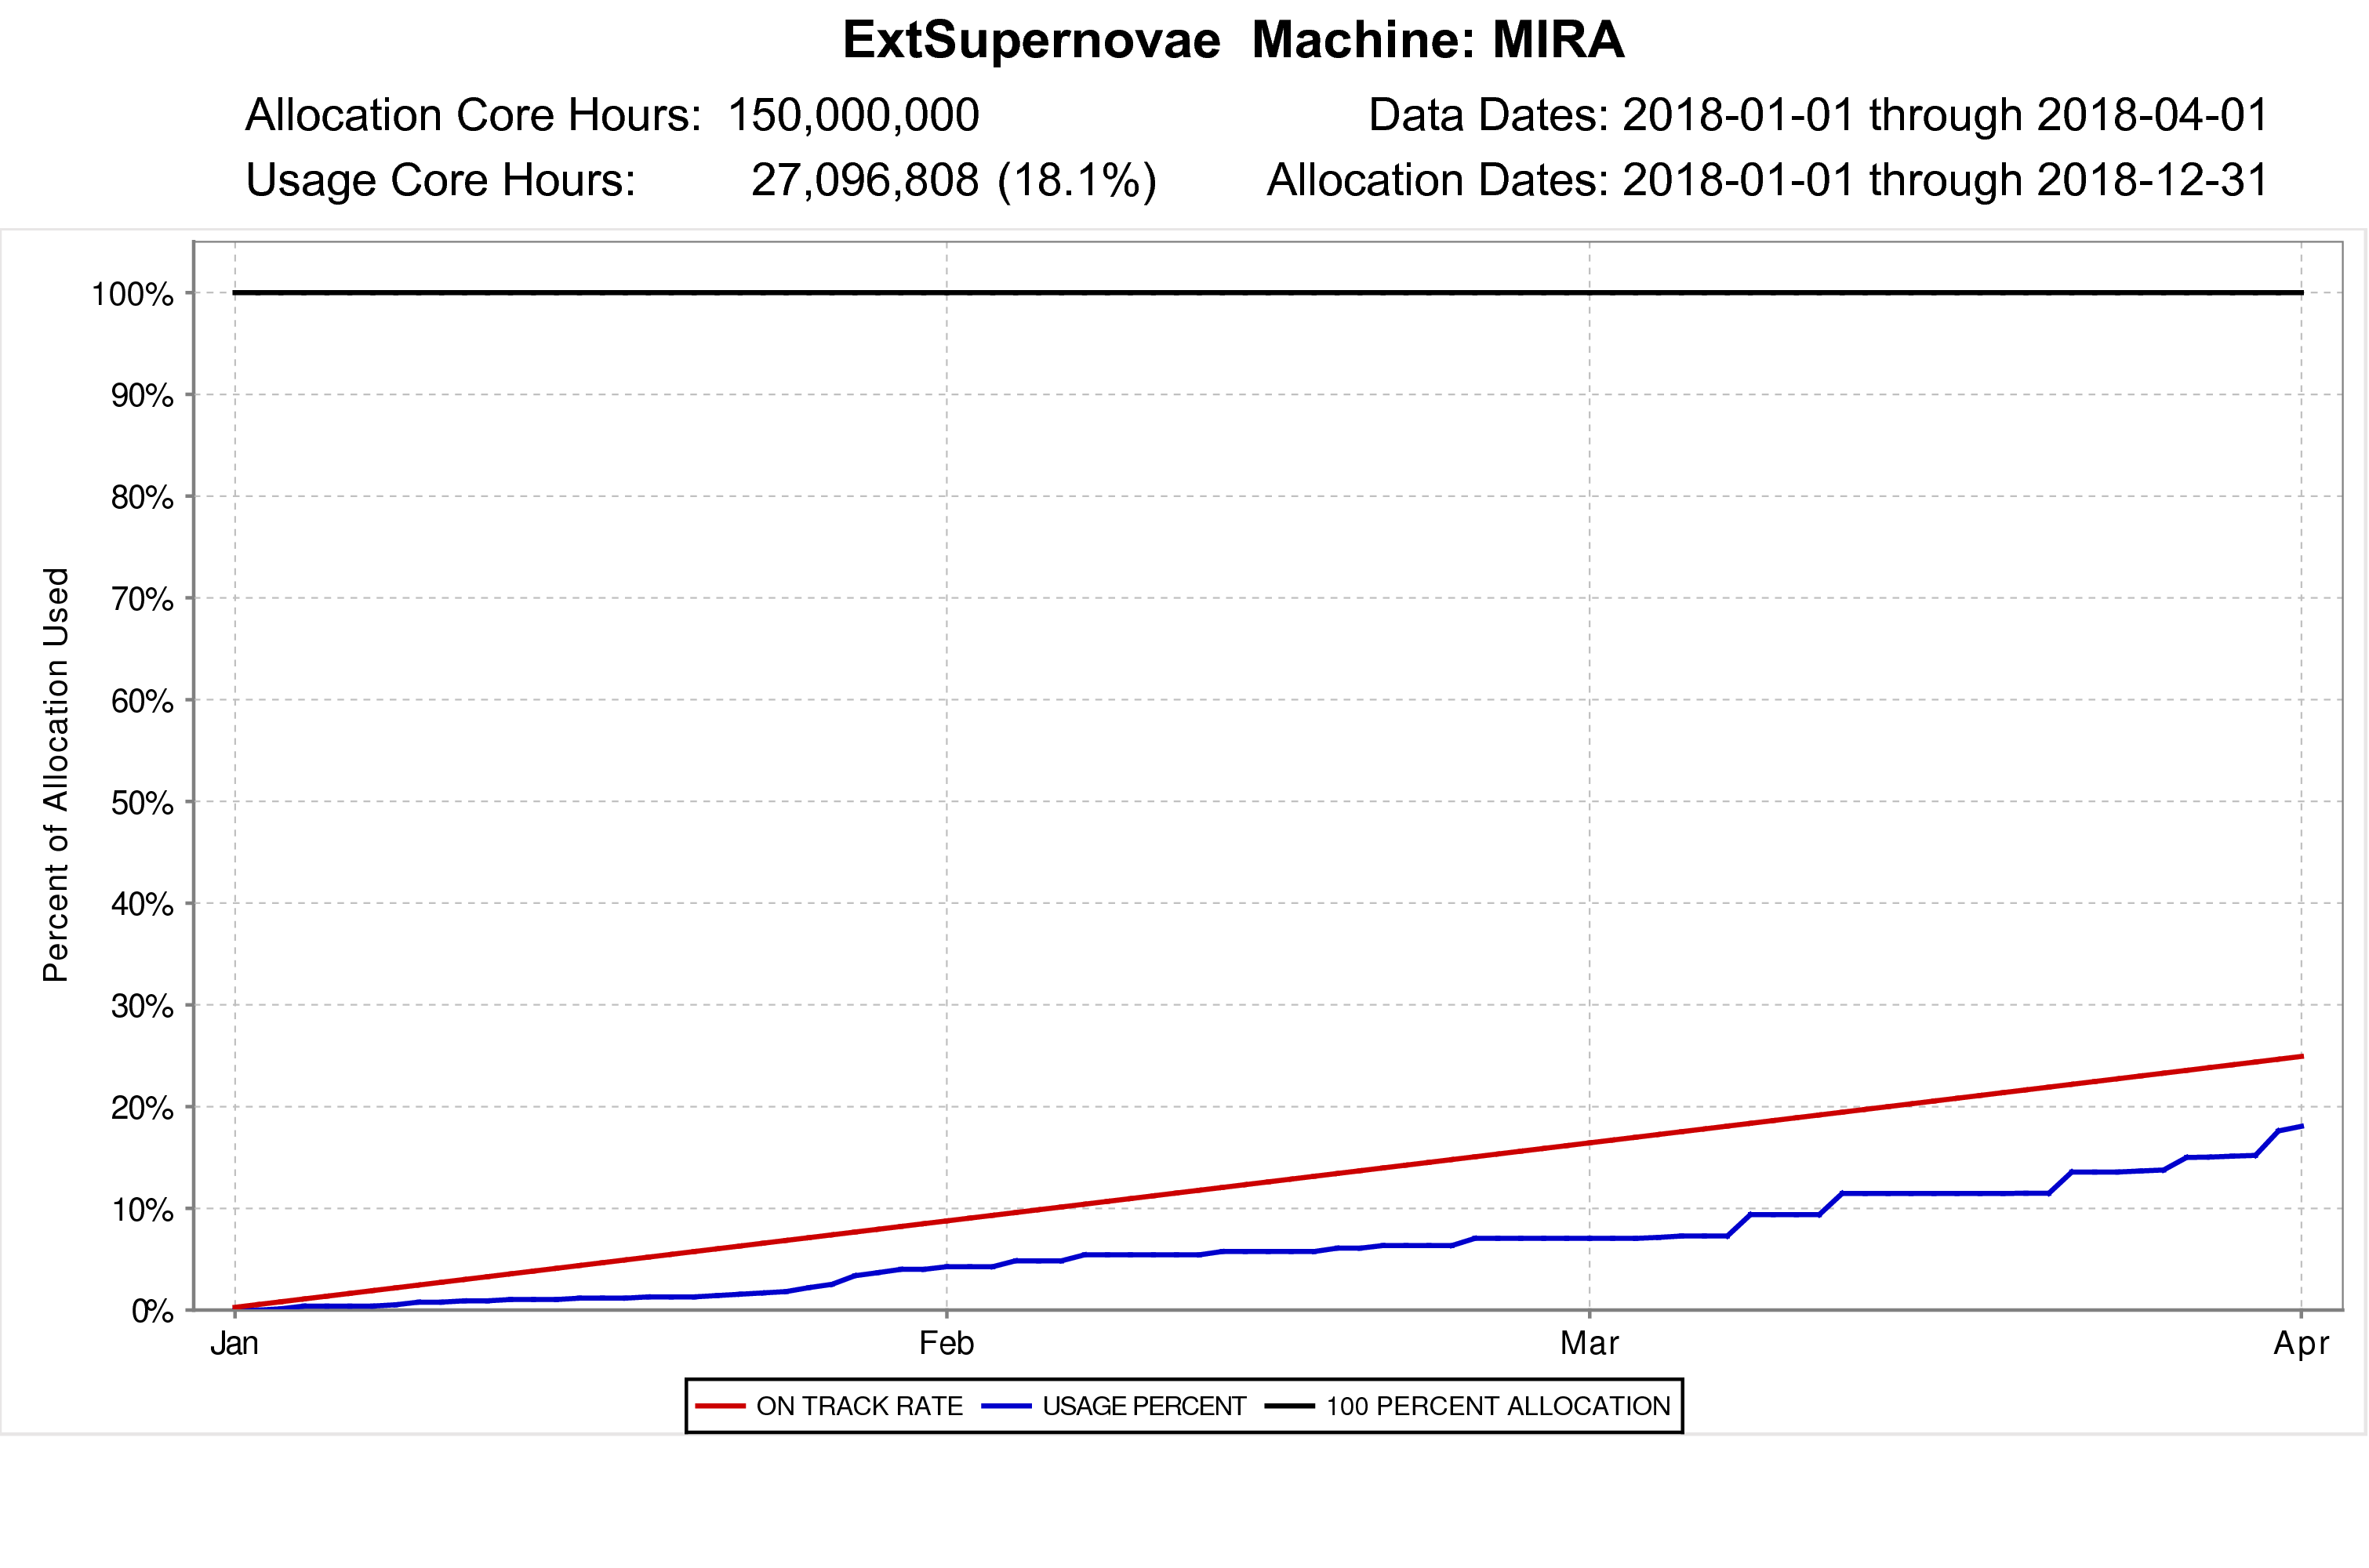
\includegraphics[width=3.25in]{on_track_graph.png}
    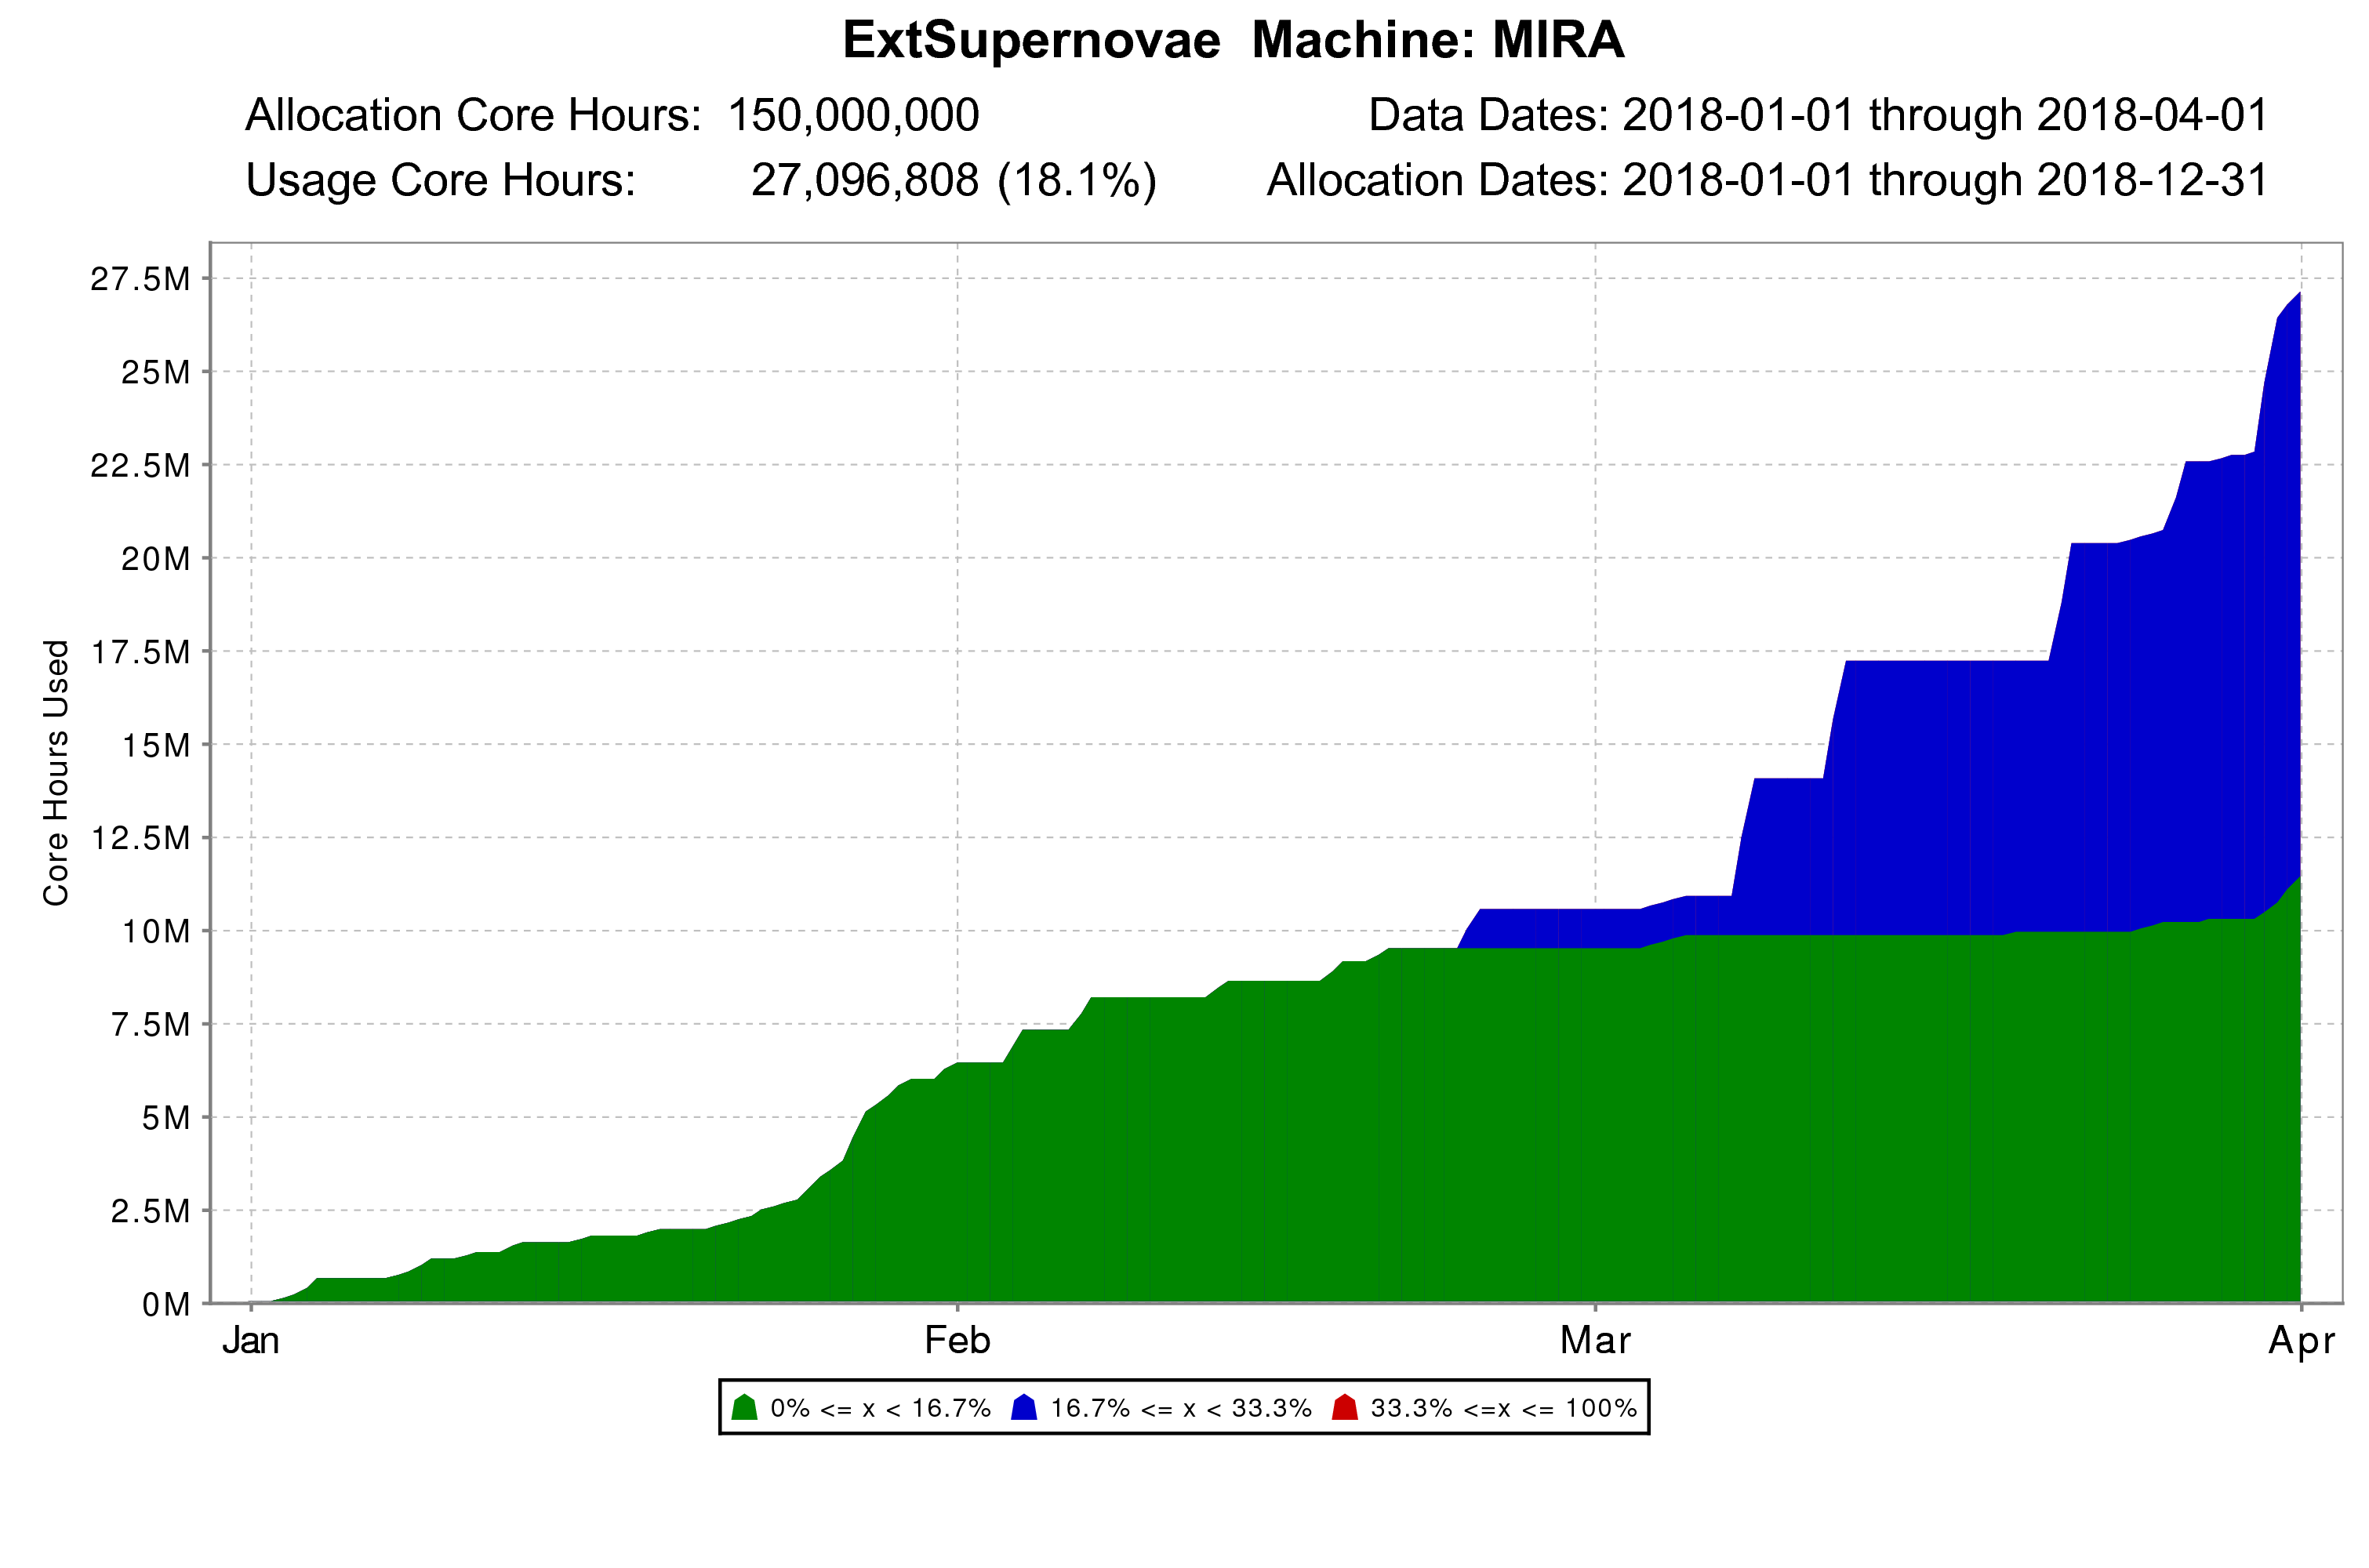
\includegraphics[width=3.25in]{categorized_hours_graph.png}
  \end{tabular}
  \caption{Allocation usage.}
  \label{fig:usage}
\end{figure}

In Q1 we have used 27.1M core-hours on Mira.
This is 18.1\% of our allocation, putting us slightly behind the ideal usage curve.
A slow start was expected since the simulations we are running grow in expense with time.
This fact is also reflected in our categorized hours (Figure \ref{fig:usage}).
As of about March 1, our simulations are now large enough to scale to the capability queue and our usage rate is now increasing substantially.

On Theta, we have expended only 1.8\% of our allocation.
This is because we have spent this quarter tuning our application for the new architecture.
We are now satisfied with the performance of our application and are ready to begin production runs on Theta.
Furthermore, we are moving one of the already-large simulations from Mira to Theta and so we should be able to run a capability scale from the outset.
We expect to dramatically increase our burn rate on Theta during Q2.




%%%%%%%%%%%%%%%%%%%%%%%%%%%%%%%%%
\section{Report on Project Milestones}
%%%%%%%%%%%%%%%%%%%

Our milestones for Year 1, and corresponding progress, are:
\begin{enumerate}
  \item {\it 3D simulations of magnetorotational core-collapse supernovae} -- These simulations have been started and are running at capability on Mira. The Theta simulations will commence in earnest in Q2.
  \item {\it 3D simulations of iron core collapse in massive stars} -- In Q1, we have optimized our simulation setup for Mira and have run preliminary simulations in reduced geometry to determine the optimal parameters and initial conditions. We plan to commence production runs in Q2.
  \item {\it High-resolution simulations of magnetorotational turbulence} -- These simulations will be started in Q2.
  \item {\it Develop SIMpliPy workflow tool} -- Work on this continues and will be accelerated in Q2. We will have two summer undergraduate REU students joining the group that will work exclusively on this tool.
  \item {\it Implement marching cubes for EOS and opacities} -- This will begin Q2 or Q3.
\end{enumerate}



%%%%%%%%%%%%%%%%%%%%%%%%%%%%%%%%%
\section{Project Productivity}
%%%%%%%%%%%%%%%%%%%

\subsection{Primary}

\noindent {\bf Publications}
\begin{itemize}
  \item \href{http://adsabs.harvard.edu/abs/2018JPhG...45e3003R}{``Turbulence in Core-Collapse Supernovae''}, Radice, D., Abdikamalov, E., Ott, C. D., Moesta, P., Couch, S. M., Roberts, L. F. 2018, {\itshape Journal of Physics G}, 45, 053003 (3 citations)
  \item \href{https://ui.adsabs.harvard.edu/#abs/2018ApJ...857...13P/abstract}{``Equation of State Dependent Dynamics and Multi-messenger Signals from Stellar-mass Black Hole Formation''}, Pan, K., Liebend\"orfer, M., Couch, S. M., Thielemann, F. 2018, {\itshape The Astrophysical Journal}, 857, 13 (4 citations)
\end{itemize}

\noindent {\bf Presentations}

\begin{itemize}
  \item ``Understanding Massive Stellar Death: Predictive Simulation of Core-collapse Supernovae,'' S.M. Couch, CCAPP Seminar, Ohio State University, Columbus, OH, April 2018
  \item ``Understanding Massive Stellar Death: Predictive Simulation of Core-collapse Supernovae,'' S.M. Couch, Physics and Astronomy Colloquium, Louisiana State University, Baton Rouge, LA, March 2018
  \item ``Understanding Massive Stellar Death: Predictive Simulation of Core-collapse Supernovae,'' S.M. Couch, Physics and Astronomy Colloquium, University of Alabama, Tuscaloosa, AL, February 2018
\end{itemize}

\subsubsection{Secondary}

\begin{itemize}
  \item Co-I and postdoc Kuo-Chuan Pan will start a faculty position at National Tsing Hua University in Taiwan this summer.
  \item Co-I and postdoc MacKenzie Warren has won a prestigious NSF Postdoctoral Fellowship.
\end{itemize}

\section{Center Feedback}

Our catalyst, Adrian Pope, has been extremely helpful.
We have been experience occasional, seemingly random, I/O errors when reading large checkpoint files at startup.
He is helping us debug this, but the error is difficult to reproduce reliably.
This has slightly slowed progress, but not ground it to a halt.


\section{Code Description and Characterization}

\texttt{FLASH} is a highly capable, fully modular, extensible,
community code that is widely used in astrophysics, cosmology, fluid
dynamics, and plasma physics, and other fields.  The capabilities of
the FLASH code include adaptive mesh refinement (AMR), several
self-gravity solvers, an advection-diffusion-reaction (ADR) flame
model, an accurate and detailed treatment of nuclear burning, and a
sophisticated two-moment neutrino transport scheme based on an
explicit hyperbolic solver.  The neutrino interactions are included
through the open-source neutrino interaction library
\texttt{NuLib}. During Year 2 of this allocation we enhanced the
performance of the two-moment neutrino transport scheme significantly
as well upgrade the transport to now include full velocity and
gravitational red-shift dependence in the evolution equations.

\texttt{FLASH} is written in modern Fortran, with some utility
functions written in C, and a build system written in Python.  It
requires MPI library support, and either HDF5 or P-NetCDF for I/O.
Additional mathematical software, such as \texttt{Hypre}, may be
required to configure \texttt{FLASH} for particular simulations.

Algorithm classes used within \texttt{FLASH} include Sparse Linear
Algebra solvers, FFT, active and passive particles, structured grids,
and AMR.



\end{document}
